%% LyX 2.3.3 created this file.  For more info, see http://www.lyx.org/.
%% Do not edit unless you really know what you are doing.
\documentclass[english]{article}
\usepackage{amsmath}
\usepackage{amsthm}
\usepackage{mathptmx}
\usepackage{newtxmath}
\renewcommand{\familydefault}{\rmdefault}
\usepackage[T1]{fontenc}
\usepackage[latin9]{inputenc}
\usepackage{geometry}
\geometry{verbose,tmargin=2.5cm,bmargin=2.5cm,lmargin=2.5cm,rmargin=2.5cm}
\PassOptionsToPackage{natbib=true}{biblatex}
\usepackage{color}
\usepackage{float}
\usepackage{graphicx}
\usepackage{setspace}
\PassOptionsToPackage{normalem}{ulem}
\usepackage{ulem}
\doublespacing

\makeatletter
%%%%%%%%%%%%%%%%%%%%%%%%%%%%%% Textclass specific LaTeX commands.
\theoremstyle{plain}
\newtheorem{thm}{\protect\theoremname}
\theoremstyle{plain}
\newtheorem{prop}[thm]{\protect\propositionname}

\@ifundefined{date}{}{\date{}}
%%%%%%%%%%%%%%%%%%%%%%%%%%%%%% User specified LaTeX commands.

\usepackage{array}
\usepackage{verbatim}
\usepackage{rotfloat}
\usepackage{booktabs}
\usepackage{bm}




%%%%%%%%%%%%%%%%%%%%%%%%%%%%%% LyX specific LaTeX commands.
%% Because html converters don't know tabularnewline
\providecommand{\tabularnewline}{\\}

%%%%%%%%%%%%%%%%%%%%%%%%%%%%%% Textclass specific LaTeX commands.






\theoremstyle{definition}
\newtheorem{definition}{Definition}[section]

\usepackage{cleveref}
\usepackage{algorithmic}
\usepackage{array}
\usepackage{stfloats}
\usepackage[super]{nth}
\usepackage{subcaption}
\usepackage{caption}
% for inkscape images
\usepackage{xcolor}
\usepackage{tikz}
\usepackage{pgf}



\g@addto@macro\@floatboxreset\centering


% \usepackage{hyperref}
 
 \AtBeginDocument{% Overrides ref for Cref
 	\let\ref\Cref
 }

\crefalias{prop}{proposition}

% TIKZ
\usepackage{tikz}


% -- Arrows
\usetikzlibrary{arrows}

% --Bayesnet
\usetikzlibrary{bayesnet}
\usetikzlibrary{decorations.pathreplacing}

\tikzset{
	diagonal fill/.style 2 args={fill=#2, path picture={
			\fill[#1, sharp corners] (path picture bounding box.south west) -|
			(path picture bounding box.north east) -- cycle;}},
	reversed diagonal fill/.style 2 args={fill=#2, path picture={
			\fill[#1, sharp corners] (path picture bounding box.north west) |- 
			(path picture bounding box.south east) -- cycle;}}
}

\tikzstyle{partialobs} = [latent,diagonal fill={gray!25}{gray!0}]

%\@ifundefined{showcaptionsetup}{}{%
% \PassOptionsToPackage{caption=false}{subfig}}
%\usepackage{subfig}
%\makeatother

\providecommand{\propositionname}{Proposition}
\providecommand{\theoremname}{Theorem}

%\DeclareFieldFormat[article,inbook,book,incollection,inproceedings,patent,thesis,unpublished]{citetitle}{#1}
%\DeclareFieldFormat[article,inbook,incollection,inproceedings,patent,thesis,unpublished]{title}{#1} 

\providecommand{\propositionname}{Proposition}
\providecommand{\theoremname}{Theorem}



% # PAPER SPECIFIC
\global\long\def\Tsq{T^{2}}%
\global\long\def\priordist{p_{z}}%
\global\long\def\detencoding{g_{\mbphi}}%
\global\long\def\detdecoding{f_{\mbtheta}}%
\global\long\def\encoding{q_{\mbphi}(\mbz\g\mbx)}%
\global\long\def\decoding{p_{\mbtheta}(\mbx\g\mbz)}%
\global\long\def\czero{c_{0}}%
\global\long\def\dataset{\mathcal{D}}%
\global\long\def\mbxover#1{\mbx^{(#1)}}%
\global\long\def\stdGauss{\Norm(\mbzero, \mbI)}%
\global\long\def\pdata{p_{data}(x)}%
\global\long\def\ptheta{p_{\mbtheta}}%
\global\long\def\pthetaxgivenz#1#2{\ptheta(#1 \g#2)}%
\global\long\def\qphi{q_{\mbphi}}%
\global\long\def\qphizgivenx#1#2{\qphi(#1 \g#2)}%
\global\long\def\pz{p(\mbz)}%
\global\long\def\oursacronym{SPE}%
\global\long\def\TsqKLD{T_{\mathrm{KLD}}^{2}}%
\global\long\def\QERE{Q_{\mathrm{ERE}}}%
% # TYPOGRAPHY
\global\long\def\etal{\textit{et al}. }%
\global\long\def\ie{\textit{i}.\textit{e}.}%
\global\long\def\eg{\textit{e}.\textit{g}.}%
% # PROBABILITY

\global\long\def\g{\,|\,}%
\global\long\def\gg{\,\|\,}%
\global\long\def\KL#1#2{\textrm{KL}\left(#1\gg#2\right)}%
\global\long\def\E{\mathbb{E}}%
% Expectation

% # DISTRIBUTIONS

\global\long\def\Norm{\mathcal{N}}%
% Gaussian likelihood
\global\long\def\Gam{\textrm{Gam}}%
\global\long\def\InvGam{\textrm{InvGam}}%
% # MISCELLANEOUS

\global\long\def\d#1{\ensuremath{\operatorname{d}\!{#1}}}%
\global\long\def\diag{\textrm{diag}}%
\global\long\def\supp{\textrm{supp}}%
\global\long\def\indep{\mathpalette{\independenT}{\perp}}%
\global\long\def\independenT#1#2{\mathrel{\rlap{$#1#2$}\mkern2mu  {#1#2}}}%
\global\long\def\inv{^{\raisebox{.2ex}{${\scriptscriptstyle -1}$}}}%

% # SET NOTATION
\global\long\def\R{\mathbb{R}}%
% # BOLD MATHEMATICS

\global\long\def\mba{\bm{a}}%
\global\long\def\mbb{\bm{b}}%
\global\long\def\mbc{\bm{c}}%
\global\long\def\mbd{\bm{d}}%
\global\long\def\mbe{\bm{e}}%
%\newcommand{\mbf}{\bm{f}}
\global\long\def\mbg{\bm{g}}%
\global\long\def\mbh{\bm{h}}%
\global\long\def\mbi{\bm{i}}%
\global\long\def\mbj{\bm{j}}%
\global\long\def\mbk{\bm{k}}%
\global\long\def\mbl{\bm{l}}%
\global\long\def\mbm{\bm{m}}%
\global\long\def\mbn{\bm{n}}%
\global\long\def\mbo{\bm{o}}%
\global\long\def\mbp{\bm{p}}%
\global\long\def\mbq{\bm{q}}%
\global\long\def\mbr{\bm{r}}%
\global\long\def\mbs{\bm{s}}%
\global\long\def\mbt{\bm{t}}%
\global\long\def\mbu{\bm{u}}%
\global\long\def\mbv{\bm{v}}%
\global\long\def\mbw{\bm{w}}%
\global\long\def\mbx{\bm{x}}%
\global\long\def\mby{\bm{y}}%
\global\long\def\mbz{\bm{z}}%
\global\long\def\mbA{\bm{A}}%
\global\long\def\mbB{\bm{B}}%
\global\long\def\mbC{\bm{C}}%
\global\long\def\mbD{\bm{D}}%
\global\long\def\mbE{\bm{E}}%
\global\long\def\mbF{\bm{F}}%
\global\long\def\mbG{\bm{G}}%
\global\long\def\mbH{\bm{H}}%
\global\long\def\mbI{\bm{I}}%
\global\long\def\mbJ{\bm{J}}%
\global\long\def\mbK{\bm{K}}%
\global\long\def\mbL{\bm{L}}%
\global\long\def\mbM{\bm{M}}%
\global\long\def\mbN{\bm{N}}%
\global\long\def\mbO{\bm{O}}%
\global\long\def\mbP{\bm{P}}%
\global\long\def\mbQ{\bm{Q}}%
\global\long\def\mbR{\bm{R}}%
\global\long\def\mbS{\bm{S}}%
\global\long\def\mbT{\bm{T}}%
\global\long\def\mbU{\bm{U}}%
\global\long\def\mbV{\bm{V}}%
\global\long\def\mbW{\bm{W}}%
\global\long\def\mbX{\bm{X}}%
\global\long\def\mbY{\bm{Y}}%
\global\long\def\mbZ{\bm{Z}}%
\global\long\def\mbalpha{\bm{\alpha}}%
\global\long\def\mbbeta{\bm{\beta}}%
\global\long\def\mbdelta{\bm{\delta}}%
\global\long\def\mbepsilon{\bm{\epsilon}}%
\global\long\def\mbchi{\bm{\chi}}%
\global\long\def\mbeta{\bm{\eta}}%
\global\long\def\mbgamma{\bm{\gamma}}%
\global\long\def\mbiota{\bm{\iota}}%
\global\long\def\mbkappa{\bm{\kappa}}%
\global\long\def\mblambda{\bm{\lambda}}%
\global\long\def\mbmu{\bm{\mu}}%
\global\long\def\mbnu{\bm{\nu}}%
\global\long\def\mbomega{\bm{\omega}}%
\global\long\def\mbphi{\bm{\phi}}%
\global\long\def\mbpi{\bm{\pi}}%
\global\long\def\mbpsi{\bm{\psi}}%
\global\long\def\mbrho{\bm{\rho}}%
\global\long\def\mbsigma{\bm{\sigma}}%
\global\long\def\mbtau{\bm{\tau}}%
\global\long\def\mbtheta{\bm{\theta}}%
\global\long\def\mbupsilon{\bm{\upsilon}}%
\global\long\def\mbvarepsilon{\bm{\varepsilon}}%
\global\long\def\mbvarphi{\bm{\varphi}}%
\global\long\def\mbvartheta{\bm{\vartheta}}%
\global\long\def\mbvarrho{\bm{\varrho}}%
\global\long\def\mbxi{\bm{\xi}}%
\global\long\def\mbzeta{\bm{\zeta}}%
\global\long\def\mbDelta{\bm{\Delta}}%
\global\long\def\mbGamma{\bm{\Gamma}}%
\global\long\def\mbLambda{\bm{\Lambda}}%
\global\long\def\mbOmega{\bm{\Omega}}%
\global\long\def\mbPhi{\bm{\Phi}}%
\global\long\def\mbPi{\bm{\Pi}}%
\global\long\def\mbPsi{\bm{\Psi}}%
\global\long\def\mbSigma{\bm{\Sigma}}%
\global\long\def\mbTheta{\bm{\Theta}}%
\global\long\def\mbUpsilon{\bm{\Upsilon}}%
\global\long\def\mbXi{\bm{\Xi}}%
\global\long\def\mbzero{\bm{0}}%
\global\long\def\mbone{\bm{1}}%
\global\long\def\mbtwo{\bm{2}}%
\global\long\def\mbthree{\bm{3}}%
\global\long\def\mbfour{\bm{4}}%
\global\long\def\mbfive{\bm{5}}%
\global\long\def\mbsix{\bm{6}}%
\global\long\def\mbseven{\bm{7}}%
\global\long\def\mbeight{\bm{8}}%
\global\long\def\mbnine{\bm{9}}%




 \setcounter{page}{1}

\usepackage{babel}

\makeatother

\usepackage{babel}
\usepackage[style=authoryear,isbn=false,url=false,eprint=false,minbibnames=10,maxbibnames=10,maxcitenames=3,firstinits=true]{biblatex}
\providecommand{\propositionname}{Proposition}
\providecommand{\theoremname}{Theorem}

\addbibresource{bibliography.bib}
\begin{document}
\title{Response to ``Toward a Better Monitoring Statistic for Profile Monitoring via Variational Autoencoders''}
\maketitle

\section{Overall Comments}

Your article has been reviewed by two reviewers and I, as guest-editor of the JQT Special Issue. Reports from the two reviewers are below. The decision for this article is Major Revision. Specifically, Reviewer 1 viewed the paper positively, but expressed concerns about the generalizability of your method. This reviewer asks you to consider other architectures besides convolutional neural networks to evaluate the generality of your method. Reviewer 2 was less positive. This reviewer expressed concerns about the ability for the JQT audience to understand your paper, and also points out several important technical issues that should be addressed. The guest editor did not provide a report, but agreed that the paper addresses an important topic, and is a good fit with the direction of the JQT Special Issue on Artificial Intelligence. The guest editor concurs with the technical and editorial suggestions of both reviewers. I encourage you to submit a revision of this article, and when doing so, please include a point-by-point response to each of the reviewers' concerns.

\textbf{\uline{Ans:}} We would like to thank you, guest editor, and both reviewers for spending time providing us the great comments. We have made the following major revisions to the paper to accommodate the JQT audiences. 
\begin{itemize}
\item We have added many discussions about the generalization of the proposed methods and how the methods can be generalized into other types of architectures beyond the CNNs. More disucssion is provided in the asnwer to Reviewer 1 Comment \#2. 
\item We have added an entirely new Section 3.1 \textcolor{black}{``Relationship of the Monitoring Statistics for VAE and PCA'' to link the monitoring statistics of the PCA and VAE models with a new figure to illustrate the analogy between VAE and PCA. The detailed discussion is provided in the answer to Reviewer 2 Comment \#3.} 
\item \textcolor{black}{We have added a new figure, Figure 2, to illustrate the analogy between VAE and PCA. The detailed discussion is provided in the answer to Comment \#3.} 
\item We have changed the original figure to explain the concepts of entanglement with more focus on the incorrect mapping of the latent space as follows to better explain the concept of the ``incorrect mapping of the latent space'' phenomena. The detailed \textcolor{black}{discussion} is provided in the answer to \textcolor{black}{Reviewer 2} Comment \#4 
\item We have revised Figure 3 completely in the paper to demonstrate why the ``latent space statistics'' would not work. We hope that this visual illustration would be much easier to understand for the JQT audiences. The detailed \textcolor{black}{discussion} is provided in the answer to Comment \#7. 
\item We have completely gone through the paper for another time to ensure the wordings we used are familiar to the JQT audiences.
\end{itemize}
Please see the more detailed resopnse addressing both reviewer's comments in the following sections. 

\section{Reviewer: 1}

\subsection{Major Comments}

This paper is well written and the technical details describing variational autoencoders, classical SPC monitoring, deep learning architectures and proposed statistics are well founded and nicely laid out. It is my belief that the paper, as currently written, deserves acceptance and publication in this journal. There are a few minor concerns that might enhance the applicability of the proposed methodology and are laid out below: 
\begin{enumerate}
\item Neural Network Architectures and Training: The authors propose convolutional neural networks. (CNNs) for both the encoders and decoders. The specific proposed architectures include Leaky ReLU activation functions with a negative slope of 0.2. The authors also use stochastic gradient descent with a batch size of 64 trained for 1000 epochs and a learning rate of 0.001. My main concern here is that this specific architecture might work well for certain problems but may not generalize well in all situations. I consider the authors should explain whether the proposed methodology is either robust to these hyper-parameters, or if hyperparameter optimization might be required for other problems.

\textbf{\uline{Ans:}} Thank you for these suggestive comments. First, we would like to clarify that we indeed performed a full sensitivity analysis on the selected parameters, including the number of latent dimensions and number of neurons. However, for some other parameters, including the slope in the Leaky ReLU, gradient batch size, and learning rate, we have adopted these choices given these parameters are most commonly used in the literature. These parameters have been selected and used in many literatures including the image reconstruction and image classification. Therefore, we believe these settings are general enough and can be used for other problems. 

For the number of epochs, we do keep a close look at the learning curve of both training and validation loss function. We found that 1000 epoch with learning rate of 0.001 is enough for the algorithm to converge (validation loss becomes stable at 1000 epochs). 

To justify our claim, we have made the following changes to Section 3.4: 
\begin{itemize}
\item We added the reference on which we base our CNN architecture \citep{higgins2017beta}. 
\item We added the reference for why we chose Leaky ReLU with a negative slope of 0.2 for activation \citep{radford2015unsupervised}. 
\item We added the reference on which we base the parameters for Adam optimizer \citep{KingmaB14}. 
\item We added a paragraph in which we explain the rationale behind our choice of how hyper-parameters are fixed. We claim that the selection is robust since the same setting worked well for two datasets that are drastically different: the simulation set and the case study. We state that our choices are based on the VAE convergence and we provide advice to the practitioners that if they need to make adjustments, they should do it with respect to this indicator. 
\end{itemize}
As a result, the following revision are added to Section 3.4: 

\textcolor{red}{``The sequential order of the computational graphs used for this study is summarized here. The architecture choice is directly based on the encoder-decoder architecture that was used in \citet{higgins2017beta}, except that we use Leaky ReLU with a negative slope of 0.2 as the activation, which is advised in \citet{radford2015unsupervised} for better gradient flow. The encoder outputs $2r$ nodes, which is a concatenation of the inferred posterior mean $\mbmu_{\mbphi}(\mbx)$ and variance $\diag(\mbsigma(\mbx))$, both are of length $r$. The number of epochs per training is fixed at $1000$, and the learning rate and batch size are fixed at $0.001$ and $64$, respectively, both are chosen empirically to guarantee a meaningful convergence. Adam algorithm is used for first-order gradient optimization with parameters $(\beta_{1,}\beta_{2})=(0.9,0.999)$ as advised in \citet{KingmaB14}. The model checkpoint is saved at every epoch where a better validation loss is observed. The latest checkpoint is used as the final model.}

\textcolor{red}{In our experiments, the architecture and the training conditions described above are optimized with respect to the convergence performance of the VAE objective on the in-control dataset. This is because in real life, the practitioner will not have access to out-of-control samples. Consequently, the same setting worked well for both the simulation dataset and the case study dataset we consider in this paper. This gives us confidence that the selection is robust from one set to the other. However, a different dataset might benefit from adjustments to the above conditions. The adjustments should be based on monitoring the convergence of the VAE objective, as the procedure will benefit from a better approximated in-control distribution. ''}
\item For sequence-based data other architectures could provide advantages, such as Long-Short Term Memory (LSTM) autoencoders. Variational LSTM autoencoders have been proposed in the literature. I think the authors should mention whether the proposed statistic could be obtained using other architectures (besides CNNs) for the generality of the methodology.

\textbf{\uline{Ans:}} Thank you for the suggestion. We do agree that 1D or sequence-based profiles are commonly found in the literature. For sequential profiles (e.g., time series), two alternative solutions can be used. First, one-dimensional convolutional and transposed convolutional layers can be used for encoders and decoders. In that scenario, since we are still in the realm of convolutional architectures, no further modifications are needed. 

Alternatively, a recurrent neural network-based encoder and decoder structure might be efficient at capturing sequential dependencies, as outlined in Chung et al. (2015). The recurrent layers would be used as a way to encode the sequence-dependent signal into a vector, just as convolutional layers do the same for spatially-dependent signals. Given that modification, the proposed monitoring statistics can still be used. Actually, we believe the proposed monitoring statistics of the papers can be used for other neural network architecture such as Variational LSTM encoder-decoder as well. 

In the revised manuscript, we have added the following material for the generalization of the proposed algorithm: 
\begin{itemize}
\item We added a related note for our readers in the last few paragraphs of Section 3.4 as highlighted below in red. 

\textcolor{red}{``In our experiments, the architecture and the training conditions described above are optimized with respect to the convergence performance of the VAE objective on in-control dataset. This is because in real life, the practitioner will not have access to out-of-control samples. Consequently, the same setting worked well for both the simulation dataset and the case study dataset we consider in this paper. This gives us confidence that the selection is robust from one set to the other. However, a different dataset might benefit from adjustments to the above conditions. The adjustments should be based on monitoring the convergence of the VAE objective, as the procedure will benefit from a better approximated in-control distribution.}

\textcolor{red}{We would like to emphasize that even we focus only on the image profiles in our paper by the convolutional architectures, which will be introduced to the readers in the upcoming simulation and case study sections, the monitoring statistics we proposed can be applied to other neural network structures as well such as the Long-Short Term Memory (LSTM) autoencoders, which will be left as the future work. ''}
\item We added the following discussion in the future work sections

\textcolor{red}{``For future work, we hope to extend the proposed method for other types of data format. For example, for sequential profiles (e.g. time series), one-dimensional convolutional layers or a recurrent neural network for encoder and decoder structures as outlined in can be used. ''}
\end{itemize}
\item The authors mention that the accuracy and computational feasibility of the proposed method, however for the sake of completeness briefly explain how computationally demanding is the proposed method and the computational limitations. With this comment, I am not necessarily referring to the theoretical computational complexity of VAEs, or of the profile monitoring procedure, but, for example, under a specific machine configuration and computational power, the methodology certain computational time, and if there are limits in either image size, sample size, batch size, learning rate, etc.

\textbf{Ans: }Thank you for this suggestion. We do agree that the computational time and configuration can affect the computational time. We would like to emphasize that the image size used in the case study is 64x64. Currently, we have about 3351 images in the training set. We used the batch size as 128. The learning rate is 0.0001. We would like to mention that there is no limit on the sample size and learning rate, given stochastic gradient algorithms can be used for any sample size or learning rate. However, there is a limit on the image size, which is pre-determined by the CNN architecture. If another image size is used, we need to either re-train the algorithm with another CNN architecture or resize the images. Appropriate batch size should also be used. In general, if the batch size is too large, the algorithm typically converges quite slow and more memories are actually required. In literature, the batch size of 128 is most commonly used in the literature and therefore used in the paper. Finally, we are able to achieve fast computational time with only 0.8 milliseconds per image on GeForce GTX 1080 Ti GPU, which satisfy the real-time computational need. 

Finally, we added the discussion of the computational time at the end of Section 5, which is highlighted below.

\textcolor{red}{``Finally, we report execution time on our specific machine configuration with respect to this case study. For this study, we utilized a workstation with 6-core Intel(R) Core(TM) i7-5930K CPU @ 3.50GHz CPUs and 4 GeForce GTX 1080 Ti GPUs. Neural network computations are executed on a single GPU and a single CPU core is used for image input/output and preprocessing steps such as resizing to 64-by-64 and grayscale conversion wherever needed. A single GPU has 12GB memory and the model parameters take up about 730MBs. GPUs can leverage parallel computation of multiple images, therefore, the remaining memory or GPU cores can be used to stock up images so their execution becomes parallel. An example of a batch of 128 images take up only 63MBs more space in the GPU's memory and the per image execution time is roughly 0.8 milliseconds. On the extreme case of using a single image per batch, average per image execution time is around 2 milliseconds, which satisfies the real-time computation. ''} 
\item Minor comments 
\begin{itemize}
\item Introduction, Page 3, Line 39\dots{} it normally requires many trial and error CHANGE TO it normally requires trial and error OR rephrase 
\item Methodology, Proposition 3.1, Page 12, Line 26 \dots . Where C1 and C2 and constants that doesn't depend on x CHANGE TO where C1 and C2 are constants that do not depend on x 
\item Comparison of Detection Performance of Proposed Statistics, Page 25, Line 47 \dots{} the former three is that they don't rely on random samples CHANGE TO the former three is that they do not rely on random samples. 
\end{itemize}
\textbf{\uline{Ans:}} Thank you for the detailed revision of the paper. We have made the changes accordingly and carefully proofread the rest of the paper again. All the changes are highlighted in red in the papers. 
\end{enumerate}

\section{Reviewer: 2}
\begin{enumerate}
\item I like the intuition that is conveyed regarding why (9) by itself is not a good monitoring statistic and how (10) overcomes this. My primary concern is that the paper is not written with the JQT audience in mind and assumes readers are more familiar with VAE and deep learning concepts than typical JQT readers are. I hope that the authors can improve upon this aspect, since I think it could make a nice contribution to JQT. Many of my comments below relate to this.

\textbf{\uline{Ans:}} We have revised the paper accordingly, with the consideration of the JQT audience in mind. Please see the detailed list of revisions below. 
\begin{itemize}
\item We have added a new Section 3.1 \textcolor{black}{``Relationship of the Monitoring Statistics for VAE and PCA'' to link the monitoring statistics of the PCA and VAE models. A detailed discussion is provided in the answer to Comment \#3.} 
\item \textcolor{black}{We have added a new figure, Figure 2, to illustrate the analogy between VAE and PCA. The detailed discussion is provided in the answer to Comment \#3.} 
\item We have completely change the original figure to explain the concepts of entanglement, with more focus on the incorrect mapping of the latent space as follows to better explain the concept of the ``incorrect mapping of the latent space'' phenomena. The detailed \textcolor{black}{discussion} is provided in the answer to Comment \#4 
\item We have revised Figure 3 completely in the paper to demonstrate why the ``latent space statistics'' would not work. We hope that this visual illustration would be much easier to understand for the JQT audiences. The detailed \textcolor{black}{discussion} is provided in the answer to Comment \#7. 
\item We have removed some of the original discussions about the disentanglement, which we also found misleading and hard to interpret. Moreover, we have completely rewritten Section 4.2 to better explain the ``incorrect'' mapping of the latent space with a better interpretation of Figure 5. The detailed \textcolor{black}{discussion} is provided in the answer to Comment \#8. 
\end{itemize}
\item The writing is very sloppy. Even the very first sentence of the abstract is incomplete and clearly was not proofread. There are also a lot of typos and other careless mistakes, e.g., inconsistencies in the list of references, like some names being replaced by et al. The writing must be improved to be suitable for JQT.

\textbf{\uline{Ans:}} Thank you for pointing out our writing issues. We have proofread the papers again and all the revisions of the papers are highlighted in the revised manuscript. The references are updated according to ``Taylor \& Francis US Chicago (B) author-date style''. We would like to note that you will still see et al. in the paper with the title ``DeepSpeech...'' because it has more than 10 authors and the said T\&F guide dictates et al. for papers with more than 10 authors in the references section. 
\item Even more critical than sloppy writing is that it is not written with the JQT audience in mind. For example, the three lines before EQ. (6) need elaboration. I am pretty familiar with VAEs and also with multivariate SPC, but I am still having trouble following what the authors mean. I think many JQT readers, especially those less familiar with \textquotedbl machine leaning\textquotedbl{} will not be able to follow. The same goes for much of the rest of the paper, e.g., the arguments in Section 3.1, which is really the main contribution of the paper. I was able to follow, but I had to read it a few times, and I don't think most JQT readers will do that. The writing should be more tailored to the JQT audience.

\textbf{\uline{Ans:}} Thank you for the suggestions. We do agree with your comments that some JQT audience may not be familiar with many learning concepts that we introduced in the paper.
\begin{itemize}
\item We restructured the paper substantially, especially Section 3. Before we introduce our methodology, we first start with where the JQT audiences are familiar with, which is the PCA methods. We discussed how naturally we can extend the monitoring statistics, namely the T2 and Q, to the VAE methods. We also added a new figure, Figure 2, to visually describe the logic behind this extension for a better understanding of our readers. The change of what we made in Section 3.2 is given at the end of this answer.
\item We further introduce the proposed monitoring statistics in Section 3.2. Moreover, Section 3.2 then criticizes using the latent space statistics in VAE methods without exposing the reader to overwhelming details of machine learning literature. We gave another figure Figure 3 to illustrate the reasons why latent space statistics may fail conceptually. For more details about the change, please refer back to the answer to Comment \#7. 
\end{itemize}
Here's how Section 3.1 is updated, which mainly addresses the concerns in this comment:

\textcolor{red}{``A common approach in the literature to tackle process monitoring with VAE is to extend the definitions of $\Tsq$ and $Q$ statistics of the PCA-based monitoring to VAE. This is done by breaking the tractable portion into two terms as follows:}

\textcolor{red}{
\begin{equation}
Q_{VAE}=\E_{\mbz\sim q_{\mbtheta}}\log\decoding,T_{VAE}^{2}=\KL\encoding{p(\mbz)}.\label{eq: TQVAE}
\end{equation}
}

\textcolor{red}{Either these formulations or some variant of them are typically used as the monitoring statistics. To understand the rationale behind this, we will revisit the assumptions of the model. Let us formally represent an out-of-control distribution as a shift in $p(\mbx)$. Since $p(\mbx)=\int p(\mbx\g\mbz)p(\mbz)d\mbz$, we can anticipate two sources: a shift in the latent distribution $\pz$ or a shift in the residual distribution $p(\mbx\g\mbz)$. The two statistics are assumed to be connected to these two sources: 1) a shift in the conditional distribution $p(\mbx\g\mbz)$ can be detected monitoring $Q_{VAE}=\E_{\mbz\sim q_{\mbtheta}}\log\decoding$ and 2) a shift in the latent distribution $p(\mbz)$, can be detected monitoring $T_{VAE}^{2}=\KL\encoding{p(\mbz)}$.}

\textcolor{red}{This idea is similar to utilizing both $T^{2}$ and $Q$-charts in the PCA-based method, where both terms play an important role in process monitoring \citep{kim2003process}. To make this similarity more obvious, we prove that if the same ELBO framework for VAE used above is used for PPCA, we prove the equivalency of $T^{2}$ and $Q$ statistics of PPCA and $T_{VAE}^{2}$ and $Q_{VAE}$ of VAE in the linear settings.}
\begin{prop}
\textcolor{red}{\label{prop: T2Q} If we use linear decoders for VAE, the models will become the Probabilistic PCA \citep{tipping1999probabilistic} that the prior and decoding functions are normally distributed as: 
\[
\begin{split}p(\mbz) & =\Norm(0,\mbI),\\
\decoding & =\Norm(\mbW\mbz,\sigma^{2}\mbI).\label{eq:Gaussian}
\end{split}
\]
In this case, the encoder can be solved analytically as another normal distribution as $\encoding=\Norm(\mu_{\mbphi}(\mbx),\Sigma_{z})$, where $\mu_{\mbphi}(\mbx)=\mbM^{-1}\mbW^{\top}\mbx$, $\Sigma_{z}=\sigma^{2}\mbM^{-1}$, and $\mbM=\mbW^{\top}\mbW+\sigma^{2}\mbI$. Then, the two monitoring statistics defined in \ref{eq: TQVAE} can be derived as follows: 
\begin{equation}
\KL\encoding{p(\mbz)}=\frac{1}{2}\gg\mu_{\mbphi}(\mbx)\gg^{2}+C_{1},\label{eqn:KL_PPCA}
\end{equation}
\begin{equation}
\E_{\mbz\sim q_{\mbphi}}\log\decoding\propto\gg\mbx-\mbW\mu_{\mbphi}(\mbx)\gg^{2}+C_{2},\label{eqn:E_PPCA}
\end{equation}
where $C_{1}$ and $C_{2}$ are constants that do not depend on $x$. The proof is given in the Appendix. }
\end{prop}

\textcolor{red}{Note that the constants do not affect the profile monitoring decision as the control limits will be translated accordingly. Thus, the test statistic $T_{VAE}^{2}$ and $Q_{VAE}$ for linear decoders (i.e., PPCA) is equivalent to the $T^{2}$-statistic and $Q$-statistic of PCA, respectively. residual-space}

\textcolor{red}{Observe that previously proposed formulations mentioned draw inspiration---directly or indirectly---from this framework. Statistics $R$ and $SPE$ are based on the $Q$-statistic. Let us call these }\textcolor{red}{\emph{residual-space statistics}}\textcolor{red}{, as they rely on the sum of squared differences between the signal itself and its predicted value, \ie, residuals. The statistics $H^{2},T^{2}$ and $D$ are based on the $T^{2}$ of PCA. We call these }\textcolor{red}{\emph{latent-space statistics}}\textcolor{red}{, as they rely exclusively on latent representations.}

\textcolor{red}{\ref{fig:pcaVSvae} shows a graphical illustration of this analogy of residual-space statistics and latent-space statistics for PCA and VAE. Residual-space statistics quantify the distance of the observed data with respect to the learned linear or nonlinear manifold. The latent-space statistics monitors the distance within the learned manifold. In the linear case (i.e., PCA), this is the Euclidean distance. However, in the nonlinear case (i.e., VAE), this distance should be defined on the nonlinear manifold.''}

\textcolor{red}{}
\begin{figure}[t]
\captionsetup{labelformat=empty} 
\centering{}\textcolor{red}{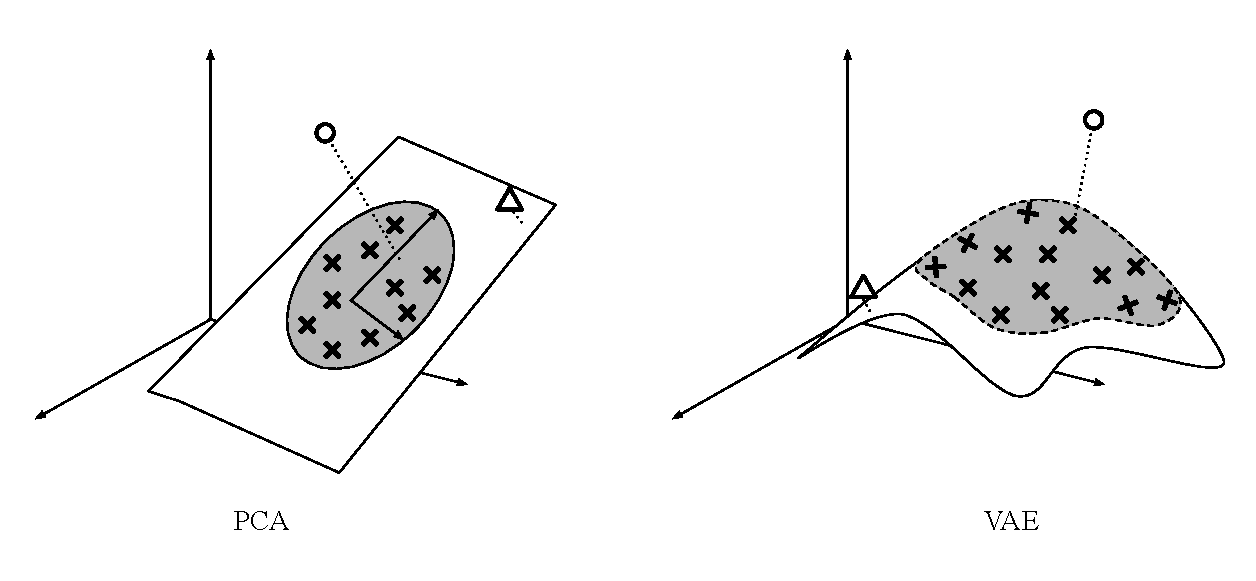
\includegraphics[width=0.9\textwidth]{PCAvsVAE} \caption{\textbf{\textcolor{red}{Figure 2 in the updated manuscript.}}\textcolor{red}{{} Illustration of the analogy between PCA and VAE. Closed regions describe the lower-dimensional manifold the in-control distribution lies in. The crosses represent the in-control samples observed in Phase-I and the gray region represents the subset of the lower-dimensional manifold where in-control samples are typically sampled from. The observation represented with a circle is typically detected with $Q$-statistic and the observation represented with a triangle is typically detected with $\Tsq$-statistic. \label{fig:pcaVSvae}}}
}
\end{figure}

\item On page 12, I recommend rewording the statement \textquotedbl Our first major claim is that latent variable-based statistics are not useful for profile monitoring ...\textquotedbl{} I think you mean that using only (9) (the T\textasciicircum 2-like component) by itself is not useful. But since (10) can also be viewed as a latent variable-based statistic, the current wording sounds like you are saying that using (9) and (10) together are not useful.

\textbf{\uline{Ans:}} Thank you for this important suggestion. Given that the models we are using belong to the latent-variable models, it is quite understandable that the word ``latent variable-based'' may cause confusion on which statistics it actually refers to, either (9) or (10). 

To make it more clear, we will use the space, in which these two monitoring statistics were computed to refer to these two statistics. Thus, we referred to the statistics (10) as the ``residual space statistics'' and the statistics (9) as the ``latent space statistics''. Section 3.1 is where we first introduce these terms to the reader, right after we make the analogy between PCA and VAE monitoring statistics. The exact change is highlighted in red below. This way, the readers will internalize the analogy between them and the $\Tsq$ and $Q$ statistics, but without getting confused about all the notations that are being thrown around. From thereafter, we consistently use these terms in the rest of the paper. 

Finally, we gave better clarification of the monitoring statistics in Section 3.1 of the paper as:\textcolor{red}{{} ``Note that the constants do not affect the profile monitoring decision as the control limits will be translated accordingly. Thus, the test statistic $T_{VAE}^{2}$ and $Q_{VAE}$ for linear decoders (i.e., PPCA) is equivalent to the $T^{2}$-statistic and $Q$-statistic of PCA, respectively. residual-space}

\textcolor{red}{Observe that previously proposed formulations mentioned draw inspiration---directly or indirectly---from this framework. Statistics $R$ and $SPE$ are based on the $Q$-statistic. Let us call these }\textcolor{red}{\emph{residual-space statistics}}\textcolor{red}{, as they rely on the sum of squared differences between the signal itself and its predicted value, \ie, residuals. The statistics $H^{2},T^{2}$ and $D$ are based on the $T^{2}$ of PCA. We call these }\textcolor{red}{\emph{latent-space statistics}}\textcolor{red}{, as they rely exclusively on latent representations..''}
\item Why are you considering a VAE, as opposed to just an AE, i.e., why do we need the variational part? By this, I mean why shouldn't we omit any assumed distribution p(z) and just fit a regular autoencoder? With a regular AE, we still have the encoded variables $z=\mu_{\phi}(x)$, the decoded approximation $\mu_{\theta}(z)$, and the \textquotedbl residuals\textquotedbl{} $x-\mu_{\theta}(z)$, so we could still consider the same two $T^{2}$-like monitoring statistics for z and for the residuals. As I mention in a comment below, I suspect part of the reason for the failure-to-extrapolate is that the assumed p(z) acts like a regularizer and prevents some of the z's from falling outside the normal region, even when the x falls outside its region. Maybe you would not have this failure-to-extrapolate problem if you use a regular AE instead of a VAE.

\textbf{\uline{Ans:}} Thank you for this comment. The major issue of using a regular AE is the irregular latent space mapping and the challenge of setting the decision boundary around this prior-free cloud of points related to the latent-space statistics.

For example, one can think of a number of alternatives: (1) fitting a multivariate Gaussian, (2) using a minimum enclosing hyperrectangle (whether axis-parallel or arbitrarily oriented), (3) using average distance to K-nearest neighbors or (4) fitting a Kernel density estimation model. All these alternatives come with an implicit assumption around the distribution of the in-control samples. More often than not, it is very unlikely to hard to guess which one will work best for any given dataset, especially when deep learning-based encoder-decoder structures are used against very complicated datasets such as images.

To illustrate the ineffectiveness of the AE method, we ran another set of experiments. For fairness, we kept the same convolutional encoder-decoder architecture as in VAE for the real-case study. The experiments were run on the same train-validation-test split of the rolling image dataset. We plot the encoded variables $z=\mu_{\phi}(x)$ below for when the compressed length is 2, similar to the way we did it in the paper. We also provide some decision boundary alternative in line with our discussion above. We can observe that using regular AE does not necessarily mitigate the issue in question. Other than classes 3, 5 and 6, none of the class encodings (shown in blue) really deviate too much from the center of gravity of the validation points (shown in red). Classes 3, 5 and 6 are not surprising either. They are the ones that are picked up the most by latent space statistics (please see column $H^{2}$ in Table 3 in page 28 of the old manuscript or Table 3 of the new manuscript). This suggests that AE and VAE behave quite similar regardless of the regularization brought up by VAE. Overall, we like to conclude that the lack of the extrapolation issue is an inherent problem of deep neural networks, including both VAE and AE, which has been discussed in Appendix B. As a result, we would like to emphasize that the regularization provided by the VAE method is not the root cause of the bad performance of the latent-space statistics.

Finally, we would like to mention that the advantage of the anomaly detection performance for the VAE method compared to the AE method has been proved in many papers, including \citep{an2015variational}, which is not the major focus of this paper. In this paper, we emphasize more on finding the most efficient and effective statistic for VAE methods, which have been proved to be very useful for anomaly detection in literature \citep{an2015variational}.

\begin{figure}[H]
\captionsetup{labelformat=empty} 

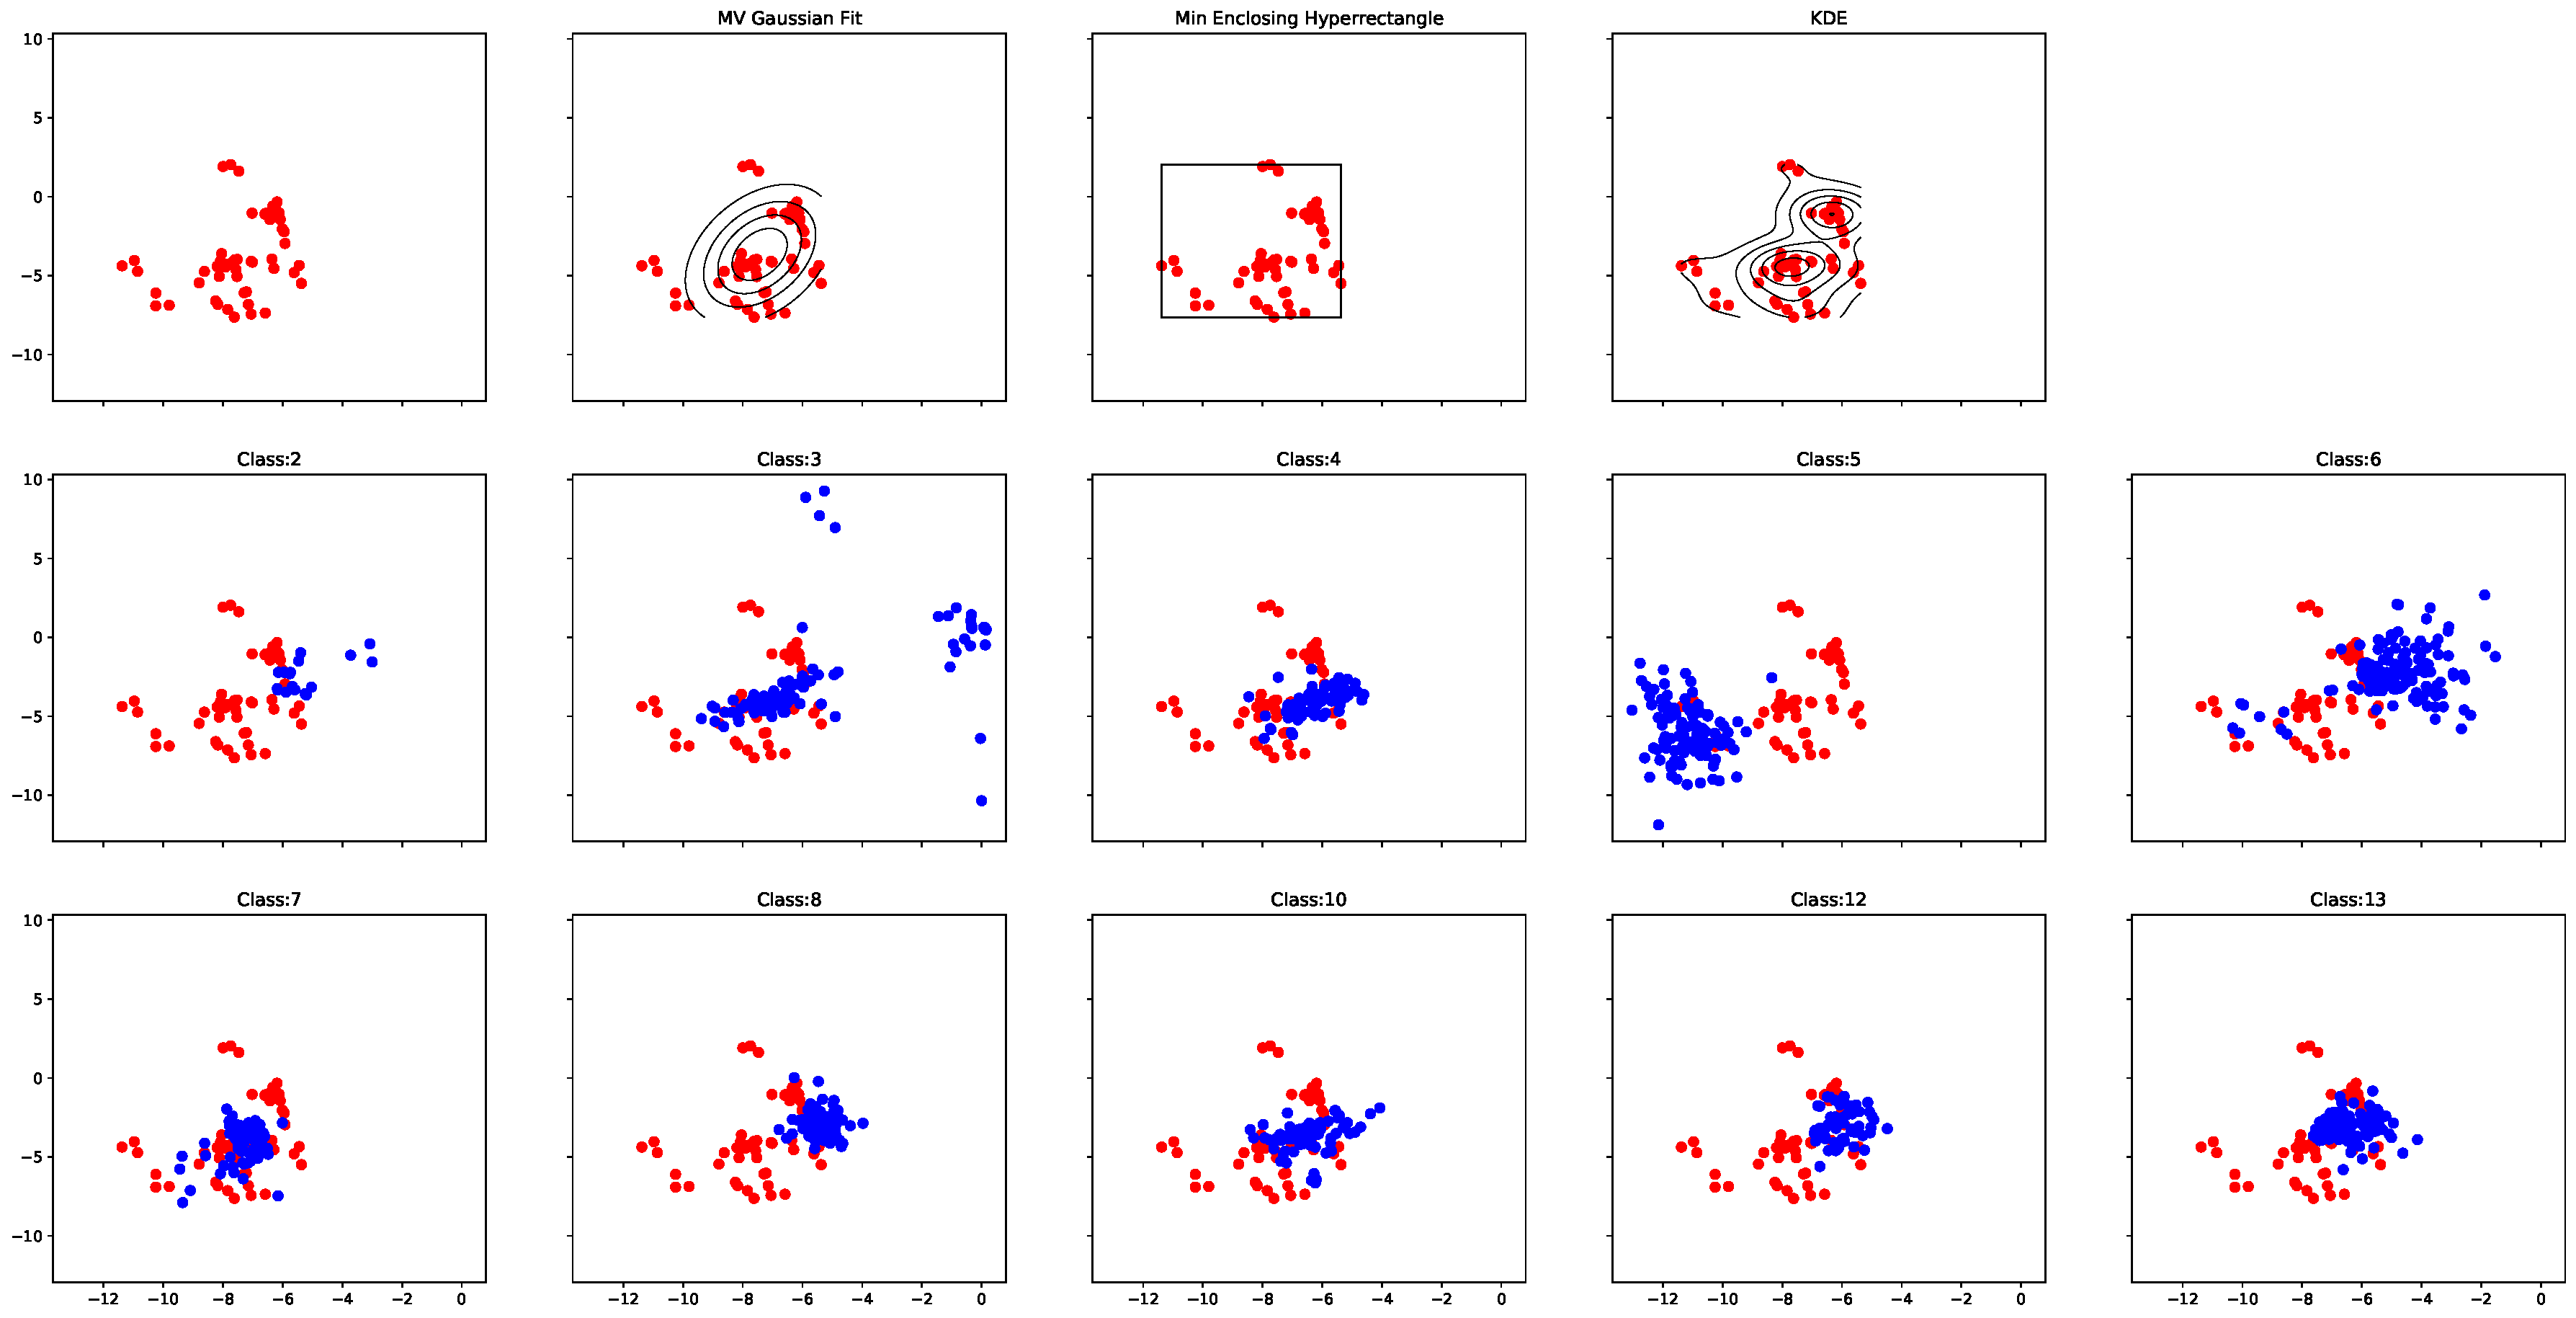
\includegraphics[scale=0.2]{scatter}

\caption{Encoded variables with a regular AE. Validation samples are shown in red. Out-of-control class samples are shown in blue. Black lines indicate the contours of the fit wherever applicable.}
\end{figure}

\item Regarding point 1 on page 12: For the standard linear PCA-based monitoring, it is well known that only monitoring the dominant PC space misses shifts that occur outside of this space. I recommend including an older reference on this, and relating your point to the analogous point for linear PCA. This will help JQT readers (who are familiar with the linear situation) to better relate to the nonlinear situation.

\textbf{\uline{Ans:}} Thank you for this comment. The argument you are referring to in your comment roughly refers to using $Q$ alongside with $\Tsq$ because $\Tsq$ by itself is not enough for monitoring with PCA, which is indeed correct. We have added the following reference in the paper \citep{Chen2004-px} to illustrate that both $\Tsq$ and Q statistics are needed for PCA methods. 

Furthermore, we have added an entirely new section 3.1 with Figure 2 to illustrate the connection of $\Tsq$ and $Q$ in PCA and $T_{VAE}^{2}$ and $Q_{VAE}$ in VAE. We would like to emphasize that despite all the similarities mentioned in section 3.1, there are actually several important differences, which we argued in Section 3.2.  

The argument we make in this paper takes this argument further and suggests that if VAE used instead of PCA, only $Q$ should be used. Therefore, especially in Section 3.2, we focused on why $\Tsq$-like statistics (\ie, latent space statistics) are unreliable, which we relate to the incorrect latent mappings produced by VAE. The probabilistic equivalent of "monitoring dominant PC shifts" is what we explain in the paper as monitoring the shift in the prior distribution $\pz$. Unlike how previous papers claim, latent-space statistics cannot be trusted to detect such shifts. Instead, residual space statistics can do that too, in addition to being able to detect shifts in the condition distribution $p(\mbx\g\mbz)$. To reflect this change, we added a new, more concise enumeration of our argument in the introduction part of Section 3.2: 

\textcolor{red}{``There are two major pitfalls of the previously proposed methodologies: }
\begin{enumerate}
\item \textcolor{red}{Latent-space statistics $H^{2},T^{2}$ and $D$ or any other formulation that relies exclusively on the latent representation $\mbz\sim\qphizgivenx\mbz\mbx$ will be unreliable for process monitoring. Thus, they should be discarded altogether from the monitoring framework since they will likely increase false alarms without contributing to the detection power in any meaningful way. }
\item \textcolor{red}{Residual-space statistics $SPE$ and $R$ rely on Monte Carlo sampling. These are not computationally feasible given how expensive calculations are on deep neural networks. An alternative approach is required to stay computationally feasible without sacrificing too much from the estimation quality of these statistics. ''}
\end{enumerate}
\item Figure 2 and Point 2 on page 13 needs a lot more elaboration. It is making an important argument, but I don't think readers without strong machine learning background will follow with the current level of detail.

\textbf{\uline{Ans:}} Thank you for this suggestion. We agree that the original Figure 2 in our paper is not clear enough, especially for readers without a strong machine learning background. Therefore, we have made the following changes
\begin{itemize}
\item We substituted Figure 2, which is now Figure 3 in the paper. We also include that figure below for your convenience. 
\item In line with your comments about the paper being accessible by JQT audience, we also skimmed the details about the properties of latent representations, such as disentanglement or invariance to nuisance factors. 
\item The main idea that we want to convey to the readers in that section is the unreliability of the semantics of deep encoder learned latent representations when it comes to profile monitoring. 
\end{itemize}
To address this, with the help of the new figure, we updated Section 3.2.1, which is highlighted below: 

\textcolor{red}{``First, we focus on the unreliability of latent-space statistics. Let us first start with the case when the shift occurs in the latent distribution (i.e., $\pz$). According to the PCA-VAE analogy illustrated in \ref{fig:pcaVSvae}, latent-space statistics are supposed to catch such shifts, which are represented with triangular points in the same figure. While this may work for PCA-based monitoring, we claim that such an analogy cannot be straightforwardly made for VAE because neural network-based encoders in autoencoder architectures typically learn incorrect mappings of actual latent variations. We illustrate this phenomenon in \ref{fig:entang-extrap}. The line segment ABC illustrates a traversal along a latent dimension. All the samples generated along the line segment AB are sampled from the typical region of the in-control process and their mappings are contained within the typical region of the predicted space. However, Point C is generated by an out-of-control process where there is a shift in the latent distribution but its mapping incorrectly falls within the probable region. This leads to false evidence which suggests that Point C is unlikely to be generated by an out-of-control process while in reality, it was.}

\textcolor{red}{The reasons as to why incorrect mappings are learned by deep autoencoders have been studied well in the deep learning literature. Interested readers are encouraged to refer to \citet{AchilleS18} for a discussion of the properties of ideal latent representations and to \citet{locatello2018challenging} for a discussion of the challenges around attaining one of these properties, namely, disentanglement. The key takeaway is that it is very likely that we end up with an imperfect mapping, especially with real-life datasets. Consequently, in Phase-II, samples generated by out-of-control processes that are characterized by a shift in the latent distribution will not be mapped consistently to the regions in the latent space, which we consider to be unusual. This will result in an increased type-II error.}

\textcolor{red}{A natural question to ask at this point is how we should expect to detect shifts in latent distribution if we cannot rely on latent representations. We argue that the residual-space statistics (i.e, an analogue of a $Q$-chart) would catch such shifts too, even though its original purpose is to catch shifts in the residual space. Our argument is based on another "shortcoming" of neural networks, namely, failure to extrapolate. Deep neural networks approximate well only at a bounded domain defined by where the training set is densely samples from. In the context of our problem, this refers to the high-density region of $p(\mbx)$, which generated the set of in-control profiles we use in Phase-I. The behavior of the function is unpredictable and often erroneous outside the training domain. In other words, it does not extrapolate well beyond the domain of training samples, which are likely to be coming from out-of-control processes. We refer interested readers to, where we replicate this phenomenon on a toy example.}

\textcolor{red}{A decoder that fails to extrapolate is counter-intuitively helpful for the residual-space statistics since it will struggle with generating profiles that are in the low-density region of the in-control data distribution $p(\mbx)$. This means that the discrepancy between the true profile and its generated counterpart will be larger for out-of-control profiles than it is for in-control profiles, regardless of the source of the shift. Overall, we conclude that the residual-space monitoring statistic would be efficient at detecting changes in the residual space and latent space. We refer the readers to \ref{fig:entang-extrap} for an illustration. Point C is generated from a shift in the latent space distribution. However, due to the "incorrect" mapping of the latent distribution, Point C' will still lie in the in-control region of the latent space. There is a significant discrepancy between Point C and reconstruction C', which can be detected by the residual-space statistics. Point D is generated from a shift in the residual space and can be captured by the residual space statistics. In conclusion, the residual-space statistic should be able to catch both types of shifts.''}

\begin{figure}[h]
\captionsetup{labelformat=empty} 
\begin{centering}
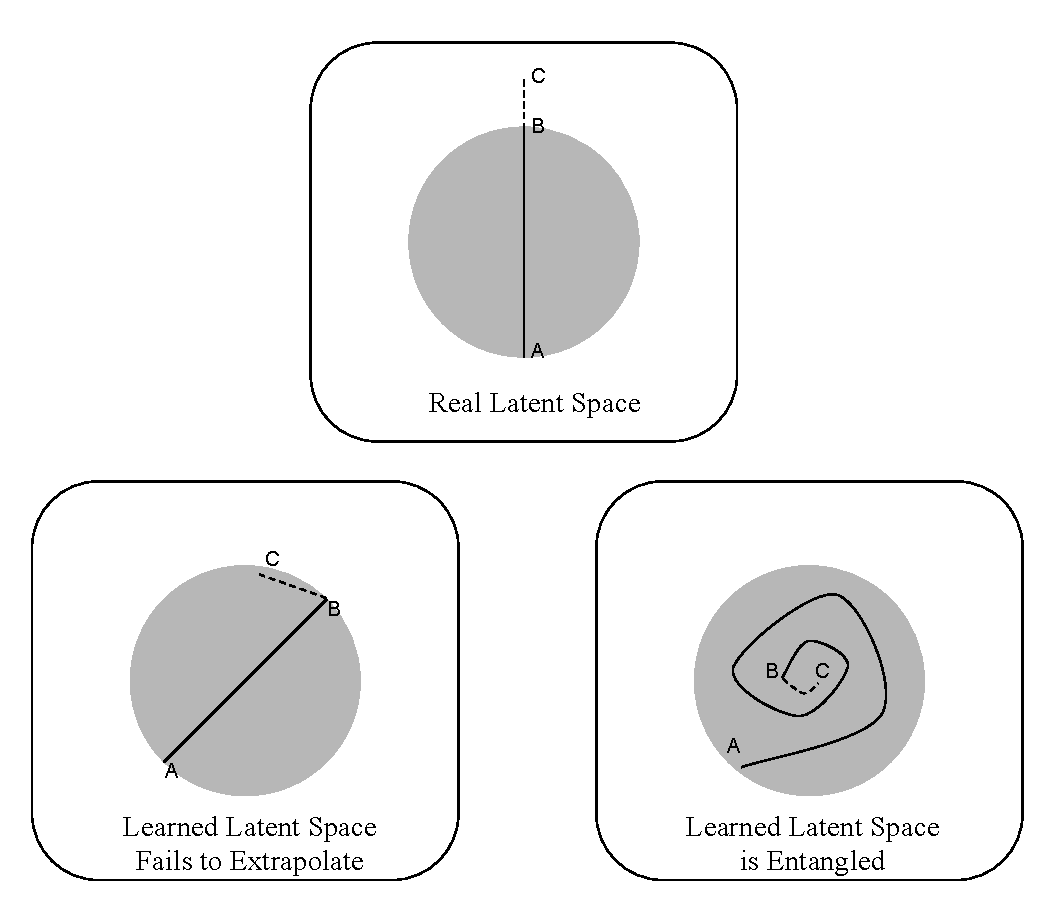
\includegraphics[width=0.9\textwidth]{Disentangled_Extrapolated} 
\par\end{centering}
\caption{\textbf{\textcolor{red}{Figure 3 in the updated manuscript.}}\textcolor{red}{{} Illustration of incorrect latent representation phenomena and how process control fails in latent space. }\textbf{\textcolor{red}{Bottom left:}}\textcolor{red}{{} The true latent variations of in-control samples are generated from the gray region, which is the probable region. Point A and Point B are extreme values along a dimension of variation. Point C is generated by an out-of-control process with a shift in latent distribution. Point D is generated by an out-of-control process with a shift in the residual distribution. The predicted counterpart of each point is denoted by an apostrophe (\eg, A' for A). }\textbf{\textcolor{red}{Top Left:}}\textcolor{red}{{} Observations of true latent variation in the high-dimensional space that lie close to a low-dimensional manifold. }\textbf{\textcolor{red}{Top Middle:}}\textcolor{red}{{} The encoder and decoder of VAE trained exclusively with in-control samples (\ie, the gray region in the observed space). }\textbf{\textcolor{red}{Bottom Middle:}}\textcolor{red}{{} Incorrectly mapped variation in the predicted latent space where the gray region is the probable region. }\textbf{\textcolor{red}{Top Right:}}\textcolor{red}{{} Reconstructions of the variation in high-dimensions, with a failure in extrapolation beyond the in-control region. \label{fig:entang-extrap}}}
\end{figure}

\item Further regarding Point 2: The crux of the failure-to-extrapolate issue is that unusual x values might get mapped to typical z values, and therefore cause false negatives. Is this because of the structure of the decoder part (which might suggest a different structure could be more suitable for this type of VAE-based process monitoring), or is it because of the implicit regularization of z when fitting the VAE via the assumed p(z), or both. I suspect the latter is just as important if not more important, but Appendix B focuses on the former. Could this problem be solved by using a regular AE instead of a VAE (per my earlier comment)? Or could it be solved by replacing the Gaussian p(z) that is used during the fitting stage with a heavier tailed distribution (e.g. multivariate t, or mixture of Gaussian and uniform over a much larger support) during the monitoring stage? If the same Gaussian p(z) is used during monitoring as during fitting the VAE, this is like telling the control chart that you expect the data during monitoring to behave the same as the data during fitting, i.e., that process shifts are not likely to happen. The Gaussian/uniform mixture p(z) would allow you to specify \textquotedbl prior\textquotedbl{} probabilities on how likely a shift is to occur.

\textbf{\uline{Ans:}} Thank you for these comments. We understand that the comments asked about if we change the prior distribution $p(z)$ to another distribution, would it help for the anomaly detection performance. We would like to answer your questions in two different angles depending on whether we would like to change the prior distribution $p(z)$ in the training stage or monitoring stage. 
\begin{itemize}
\item If you suggest change $p(z)$ to another distribution only in the monitoring stage (Phase II) but keep the $p(z)$ as the standard normal in the training stage (Phase I). I would like to mention that it is mathematically not possible to use a different distribution for the monitoring stage compared to the training stages. The purpose of Phase-II monitoring is to check if an incoming profile adheres to the in-control behavior or the same distribution learned in the Phase-I analysis with a specific $p(z)$. Besides, the encoder-decoder architecture limits you to the initial distribution you fitted it with. The typical VAE can includes an encoder that produce a mean and a diagonal covariance matrix for a Gaussian distribution, and a decoder generates the samples from such Gaussian distributions. The entire ELBO loss function depends on the Gaussian assumption, which is impossible to change without completely changing the training stage. 
\item If you are suggesting replacing Gaussian prior altogether in both Phase I and Phase II stage or at training and monitoring stages. We will need to propose a completely new model rather than the standard VAE, given the KL-divergence regularization (or any other distance measure) between the proposed prior (like t-distribution) and encoded distribution is needed. First, we need to assume that when choosing such distribution, this KL-divergence yield an analytical and differentiable formulation. For the sake of discussion, let us assume that this is not a problem. We would still like to argue that this entire new VAE method will still not help improve the performance of latent-space statistics for the following two reasons: 
\begin{itemize}
\item If we replaced $p(z)$ with a heavier-tailed distribution, the inferred means of in-control and out-of-control samples will still lies inside this particular heavy tail distribution or mixture distribution given the extropalation issue as discussed in the papers. The neural network would not learned to map the new samples into the new latent space that have not appeared in the training dataset before.
\item In general, VAE puts strong regularization as the gaussian prior. t-distribution or other heavy tail distributions put a weaker regularization. When we compare VAE and regular AEs, we conclude that even without any regularizations, the latent-space statistics still would not help. We further emphasize that the regularization we applied in VAE is not the major reasons why latent space statistics won't work. The major reasons lie into the limitation of deep neural network failed to generalize beyond the bounded regions of the training dataset. 
\end{itemize}
\end{itemize}
In the revised manuscript, we have added the following paragraph to clarify: `` \textcolor{red}{Here, we will explain the two major reasons why the latent-space statistics failed to capture the change in the latent space: \textquotedbl incorrect\textquotedbl{} latent representation by the encoder and failure to extrapolate by the decoder. }'' We then introduce these two major reasons in details in the rest of the Section 3.2.1. 
\item Section 4.1: I don't recognize this as the gasket bead example from Shi, Apley and Runger (2016). It might represent some other type of bead that changes position/shape, but it doesn't seem to have much connection to gaskets.

\textbf{\uline{Ans:}} Thank you for this comment. It is our mistake that we kept the wording gasket bead because just as your comment suggests, a 2D point cloud with a circular shape does not have much connection to the gasket bead component anymore, even though the semantics of location and shape variations have similarities. As a response: We made sure all the related wordings are changed to dome, which is a better descriptor of the topology of our simulation generating process. 
\item Additional comments that are minor by themselves but related to the bigger problem of poor writing in general: 
\begin{itemize}
\item First paragraph of intro: In \textquotedbl ... intra-sample variation lies on a nonlinear low-dimensional manifold\textquotedbl{} it is not clear what \textquotedbl sample\textquotedbl{} means. Does \textquotedbl intra-sample variation\textquotedbl{} just mean variation across a sample of parts, items, images, etc? Please clarify.

\textbf{\uline{Ans:}} Thank you for this comment. You are right to call out ``sample'' as an ambiguous word. In that sentence, we mean profile-to-profile variation. Therefore, we made the following change: 

\textcolor{red}{Specifically, we focus on the case where profiles are observed in a high-dimensional space but profile-to-profile variation lie on a nonlinear low-dimensional manifold.} 
\item Page 5, 3rd contribution bullet: It sounds like you are saying latent variable-based monitoring should not be used, but it seems the entire paper is about latent variable-based monitoring. VAEs are latent variable models. Please clarify.

\textbf{\uline{Ans:}} Thank you for this comment. Please see our answer to you comment 4. In there, we explain how we rename this to ``latent space statistic''. We agree with your comment on this. 
\item In Eq. (5), I can't find where$\mu_{\phi}(x)$ has been defined. I can guess what it is, but readers shouldn't have to guess. There are quite a few other undefined or unclearly defined notations.

\textbf{\uline{Ans:}} Thank you for this comment. We agree that $\mu_{\phi}(x)$ was not defined. We added the following sentence to Section 2.1: 

\textcolor{red}{The encoder is modeled as another Gaussian distribution $\encoding=\Norm(\mbz;\mu_{\mbphi}(\mbx),\sigma_{\mbphi}(\mbx))$ where the mean and standard deviation of the proposal distribution are inferred via high capacity neural networks $\mu_{\mbphi}$ and $\sigma_{\mbphi}$, respectively.} 
\item On page 11, does \textquotedbl this is actually true for linear latent variable models\textquotedbl{} mean \textquotedbl this holds exactly for linear latent variable models\textquotedbl ?

\textbf{\uline{Ans:}} Thank you for this comment. We have changed this sentence as suggested.
\end{itemize}
\end{enumerate}
\printbibliography

\end{document}
